\cleardoublepage
\chapter{Nodo de Consumo (NC)}

\section{Hardware}

Los Nodos de Consumo representan el elemento ejecutivo dentro de la arquitectura distribuida del sistema propuesto. A diferencia de los esquemas de control centralizados tradicionales, estos dispositivos brindan la capacidad de procesar información local y tomar decisiones de actuación de manera autónoma con informacion de sus pares. Para cumplir con este requisito de procesamiento distribuido, se seleccionó al igual que en el caso anterior un ESP32. Esta elección no es arbitraria; sino que responde a la necesidad de contar con un procesador de alta velocidad capaz de gestionar simultáneamente el muestreo de señales en tiempo real y el protocolo de comunicación inalámbrico ESP-NOW, todo ello manteniendo un bajo costo y un consumo energético acotado.

El desarrollo del hardware del NC enfrentó el desafío de circuitos de potencia, medición de precisión e interfaz de usuario en un volumen físico restringido. El objetivo de diseño fue lograr que el dispositivo final pudiera alojarse dentro de la cajas electricas de embutir rectangulares estándar de $5 \times 10$ cm, ya existentes en la gran mayoria de instalaciones eléctricas. Para resolver esta restricción espacial sin comprometer la seguridad ni la funcionalidad, se adoptó una estrategia de diseño modular, dividiendo el circuito en dos placas apiladas de circuito impreso (PCB).

Esta arquitectura de dos niveles cumple una doble función crítica. En primer lugar, optimiza el uso del espacio disponible dentro del gabinete. En segundo lugar, y más importante, establece una barrera de seguridad entre los circuitos de alta tensión y la lógica de control. La placa inferior está dedicada en parte al manejo de la tensión de red (220 V CA) y medicion de corriente, mientras que la placa superior aloja el microcontrolador y selector de prioridad. Esta separación física reduce significativamente el riesgo de inyectar alta tension al microcontrolador y minimiza el acoplamiento o interferencias electromagneticas provenientes de la red.

En la placa inferior, denominada etapa de potencia, se encuentran los siguientes subsistemas:
\begin{itemize}
    \item \textbf{Fuente de Alimentación:} Se integró un módulo convertidor CA-CC conmutado compacto, encargado de transformar la tensión de línea de 220 V CA a una tensión continua estable de 5 V para alimentar la lógica del sistema. La estabilidad de esta fuente es vital, ya que variaciones en la tensión de alimentación podrían introducir errores en la referencia del sensor de corriente.
    \item \textbf{Actuación:} El control de la carga se realiza mediante un relé electromecánico con capacidad de conmutación de hasta 12 A a 250 V CA. Dado que las salidas digitales del microcontrolador no poseen la capacidad de corriente suficiente para excitar directamente la bobina del relé, se implementó una etapa de potencia intermedia utilizando un transistor bipolar NPN de uso general (modelo BC337) configurado como interruptor entrando en corte y saturación.
    \item \textbf{Sensor:} La medición del consumo se realizó mediante un sensor de corriente por efecto Hall lineal ACS712. Este componente ofrece una ventaja fundamental ya que proporciona aislamiento galvánico entre el conductor de corriente (que está al potencial de red) y los pines de señal. El sensor entrega una tensión analógica proporcional a la corriente instantánea que circula hacia la carga. Sin embargo, como este módulo opera a 5 V y el ESP32 tiene entradas tolerantes solo hasta 3.3 V, fue necesario interponer un divisor de tensión resistivo para adecuar los niveles de señal y proteger al microcontrolador contra sobretensiones.
\end{itemize}

Por otra parte, la placa superior concentra las funciones de control e interacción. El módulo ESP32 se monta en esta, facilitando el acceso a sus puertos de programación y depuración. Para la configuración del dispositivo, se incorporó un interruptor tipo DIP Switch de dos vías. Este componente permite al instalador o usuario asignar una dirección de prioridad binaria (de 0 a 3) al nodo de manera física, eliminando la necesidad de conectar una computadora o dispositivo para reconfigurar el software cada vez que se cambia la función del nodo. Finalmente, para brindar retroalimentación inmediata, se diseñó primero una interfaz visual compuesta por una barra de LEDs de tres colores (rojo, amarillo y verde) que se puede observar en los Anexos ~\nameref{cap:prototipado} y ~\nameref{cap:desarrollo}. Estos indicadores permitian unicamente el estado de disponibilidad energética de la microrred. Luego como se puede ver en la Figura~\ref{fig:nc} se implemento un display OLED similar al del AC con diseño en 3D para ser adaptado a una tapa estandar de cajas rectangulares de la marca Cambre, es especifico su linea Siglo XXI.

\begin{figure}[hbt!]
    \centering
    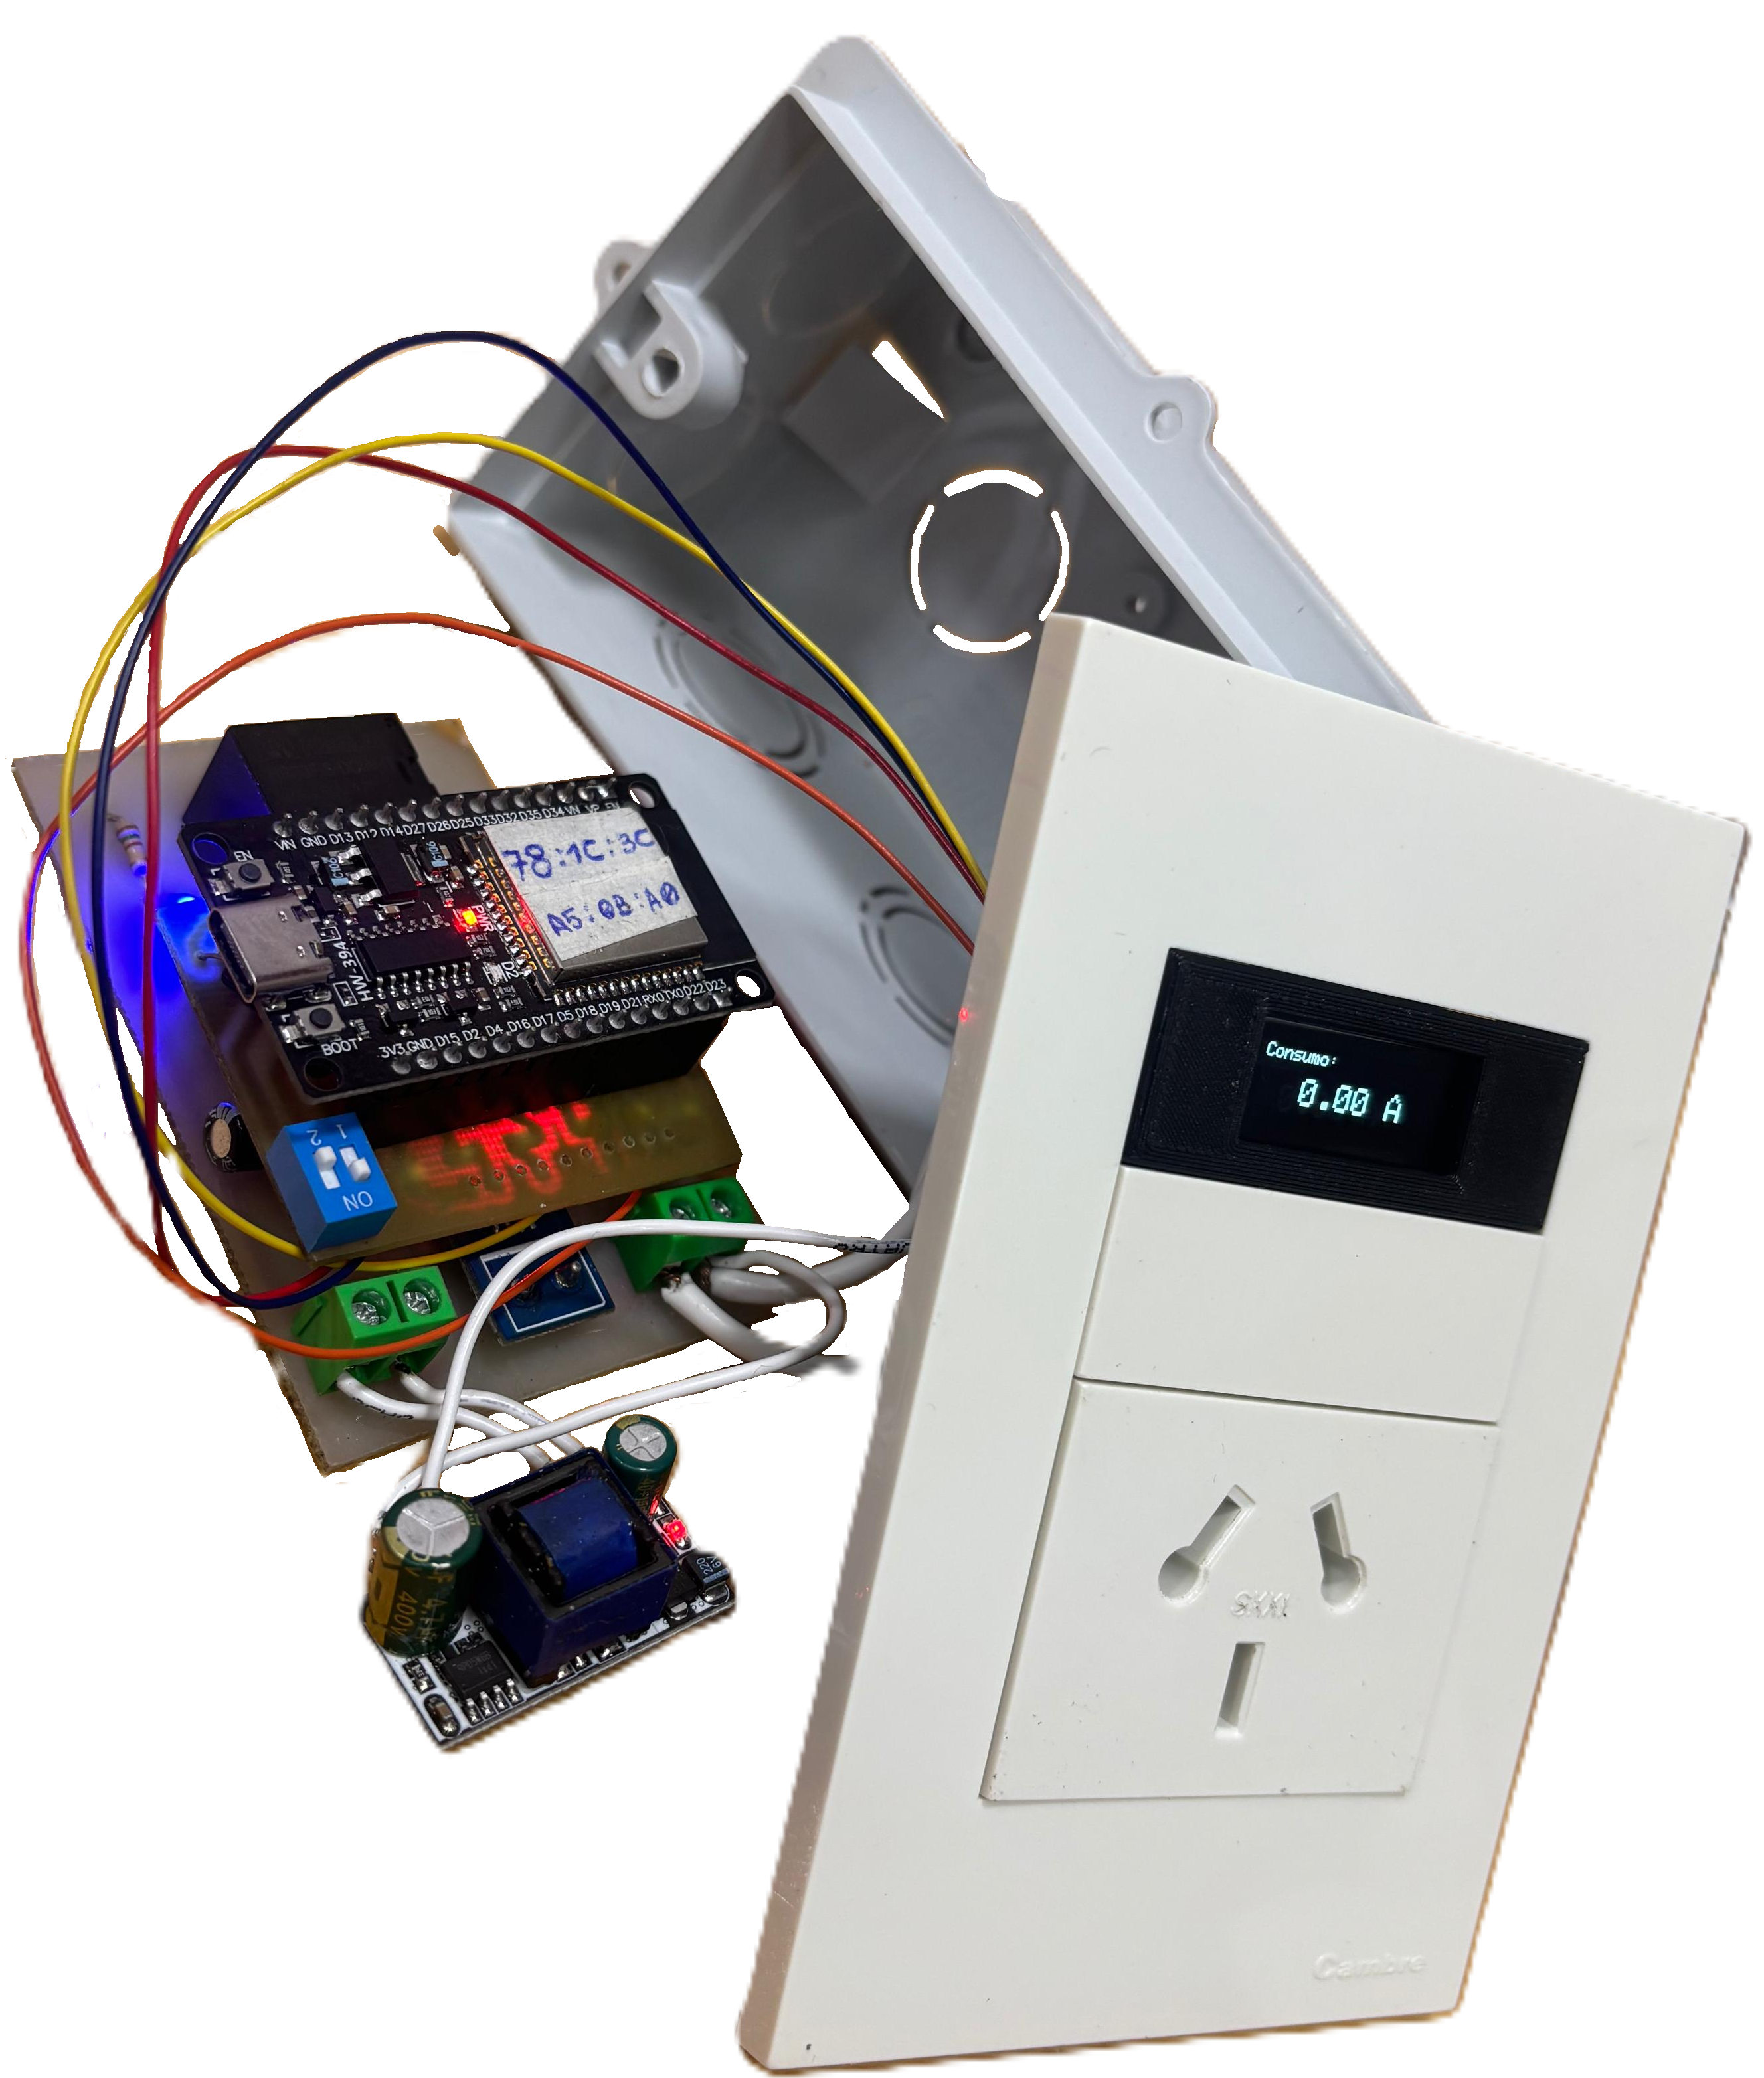
\includegraphics[width=0.6\textwidth]{imagenes/nc.jpg}
    \caption{Hardware desarrollado para el Nodo de Consumo (NC)}
    \label{fig:nc}
\end{figure}

\section{Firmware}

El firmware del NC implementa la lógica de control distribuido descrita en el Capítulo 8. Su bucle principal ejecuta tres tareas fundamentales de manera cíclica: la medición precisa del consumo, el intercambio de mensajes de consenso y la ejecución del algoritmo de decisión para la conexión o desconexión de la carga.

\subsection{Medición de Corriente}
La adquisición de la señal del sensor ACS712 sigue el mismo principio de muestreo síncrono utilizado en el AC. El microcontrolador captura la forma de onda de la corriente consumida por la carga y calcula su valor eficaz (RMS) en tiempo real.

Para validar la precisión de este método, se realizaron ensayos comparativos utilizando una punta de corriente comercial calibrada y un osciloscopio, como se muestra en la Figura~\ref{fig:prueba-corriente}. Los resultados demostraron que el sistema mantiene una linealidad adecuada y es capaz de medir correctamente incluso ante cargas no lineales (como fuentes conmutadas), reportando valores con un error en torno a los 30-40 mA siendo practicamente insignificantes respecto del valor maximo y tambien mejorable con una fuente de mayor calidad.

\begin{figure}[H]
    \centering
    \includegraphics[width=0.6\textwidth]{imagenes/prueba-corriente.jpg}
    \caption{Prueba de medición de corriente en el NC contra punta de corriente}
    \label{fig:prueba-corriente}
\end{figure}

\subsection{Lógica de Control y Actuación}
El núcleo del firmware es una máquina de estados que evalúa constantemente si la carga debe permanecer conectada o desconectada. Esta decisión se basa en la comparación entre el consumo total reportado por la red (suma de los consumos de todos los nodos) y el límite de corriente disponible informado por el AC.

\begin{itemize}
    \item \textbf{Si la carga está conectada:} El nodo verifica si el consumo total supera la disponibilidad. De ser así, y si su prioridad es la más baja de la red, procede a desconectar el relé para aliviar la carga del sistema.
    \item \textbf{Si la carga está desconectada:} El firmware aplica una lógica de reconexión con histéresis. Antes de intentar reconectar, calcula una corriente total estimada sumando el consumo actual de la red, su propio consumo histórico (guardado antes de la desconexión) y un margen de seguridad adicional. Solo si esta suma es inferior a la disponibilidad, se permite la reconexión. Esto evita oscilaciones indeseadas donde el nodo se conecta y desconecta repetidamente al estar cerca del límite.
\end{itemize}

\subsection{Interfaz de Usuario}
Para mantener al usuario informado sobre el estado operativo, el firmware gestiona un display OLED que alterna automáticamente entre diferentes vistas informativas, tal como se aprecia en la Figura~\ref{fig:pantallas}.

\begin{figure}[hbt!]
    \centering
    \subfigure[]{
        \includegraphics[width=0.2\textwidth]{imagenes/pantalla0-nc.png}
        \label{fig:pantalla0}
    }
    \hfill
    \subfigure[]{
        \includegraphics[width=0.2\textwidth]{imagenes/pantalla1-nc.png}
        \label{fig:pantalla1}
    }
    \subfigure[]{
        \includegraphics[width=0.4\textwidth]{imagenes/prioridades-nc.png}
        \label{fig:pantalla-prioridades}
    }
    \caption{Pantallas implementadas para el NC. (a) Consumo. (b) Disponibilidad. (c) Prioridades.}
    \label{fig:pantallas}
\end{figure}

\begin{itemize}
    \item \textbf{Consumo (a):} Muestra la corriente instantánea que está demandando la carga conectada al nodo.
    \item \textbf{Disponibilidad (b):} Visualiza gráficamente (mediante una barra de progreso) y numéricamente cual es la disponibilidad de la microrred.
    \item \textbf{Prioridad (c):} Indica el nivel de prioridad asignado en el hardware (Carga Crítica o No Crítica Alta, Media o Baja), permitiendo al usuario verificar la configuración del NC.
\end{itemize}